\documentclass[12p]{article}
\usepackage[utf8]{inputenc}
\usepackage[english]{babel}

\usepackage{graphicx}
\usepackage{hyperref}
\usepackage{caption}
\usepackage{mathtools}
\usepackage{lscape}
\usepackage{numprint}

\usepackage[backend=biber,style=iso-numeric,sorting=none]{biblatex}
\bibliography{references.bib}

\title{Exoplanet Ranking \\\large Introduction to Data Science}
\date{\today}
\author{Goron, Nathan\and Motzkus, Franz\and Vopat, Tomas
}

%------------------------------------------------------------------
%------------------------------------------------------------------

\begin{document}

\maketitle

\section{Introduction}

In our project we computed a ranking of the already discovered exoplanets in the pursuit of giving first sights of planets that could fit the role of next home for mankind.
Once the ranking is created, we would display it on a website, along with visualisations regarding the dataset.

We think that our study might interest companies, that want to raise people's curiosity around the topic of finding Earth-like planets, or simply astronomy enthusiast, that we can inspire with a new view.

The results of our work take form in two materials; the ranking dataset which features every exoplanet from the original dataset and, associated to each of them, a grade from 0 to 10 representing how suitable they would be as earth replacement.

%------------------------------------------------------------------

\section{Preprocessing and Analysis}
The dataset~\cite{dataset} we used is from an archive hosted by the NASA exoplanet science institute which is operated by the California Institute of Technology. In the dataset there is data about \numprint{4056} exoplanets with \numprint{47} various attributes (e.g.\ temperature, star luminosity, distance). These attributes are used to determine the ``livability score'', since they influence, if humanity could survive on this planet.

As a first step we removed the columns, that contained irrelevant information for out task such as website links or different names of the exoplanet. Next step was to drop columns with high ration of missing data. In the column \verb|fpl_eccen| is \numprint[\%]{61.7} missing and in the column \verb|fst_spt| \numprint[\%]{66.3}. As a result only \numprint{20} columns left for the ranking, these attributes are deeply described in Figure~\ref{tab:att_desc}. Since the domain knowledge of physicists, astrologists and maybe even biologists is needed, we use all the attributes mentioned above for our experiments. For further experiments it is supposed to consult with specialist the livability impact of each attribute in the dataset, as some of those might be more important than the others.

Afterwards we explored the distributions of each variable. As some of variables vary a lot, some of them are almost constant across all the dataset. To make it more clear, we plot mean value of each variable with its standard deviation in the Figure~\ref{pic:mean}. As can be seen, attributes like \verb|fst_mass| (stellar mass) or \verb|fst_lum| (stellar luminosity) have really small in comparison to others. On the other hand \verb|fst_teff| (effective temperature) and \verb|fpl_orbper| (orbit period) differ a lot. To be able to plot all the variables, it was necessary to log-scale all the values. 

Futhermore some of the variables might be correlated (mutually influenced). Due to that, we have computed correlation matrix for each pair of variables. As illustrated by Figure~\ref{pic:corr}, \verb|fst_logg| (gravity acceleration at the stellar surface) and \verb|fst_lum| (stellar luminosity) are highly correlated, which means that with the gravity acceleration the luminosity of the star decreases.

To finish the analysis, we try to group exoplanets by its properties, as the planets are situated in the vector space (not in the universe). First of all we have to normalize all the values to be in the same range (from 0 to 1). After that the clustering can be applied. We use k-means algorithm implemented in \textit{Scikit-learn}\footnote{https://scikit-learn.org} library for machine learning. It is surprising that the optimal number of clusters is \numprint{2}, since there are \numprint{4} thousand exoplanets in the dataset.

We can see in Figure~\ref{pic:cluster} that the Earth is situated in the green cluster where is \numprint[\%]{77.5} of the exoplanets. The planets are clearly distinguishable even though the space is projected by SVD (\textit{Scikit-learn}\footnotemark[\value{footnote}] implementation is used) into 2 dimensions.

\begin{figure}\centering
    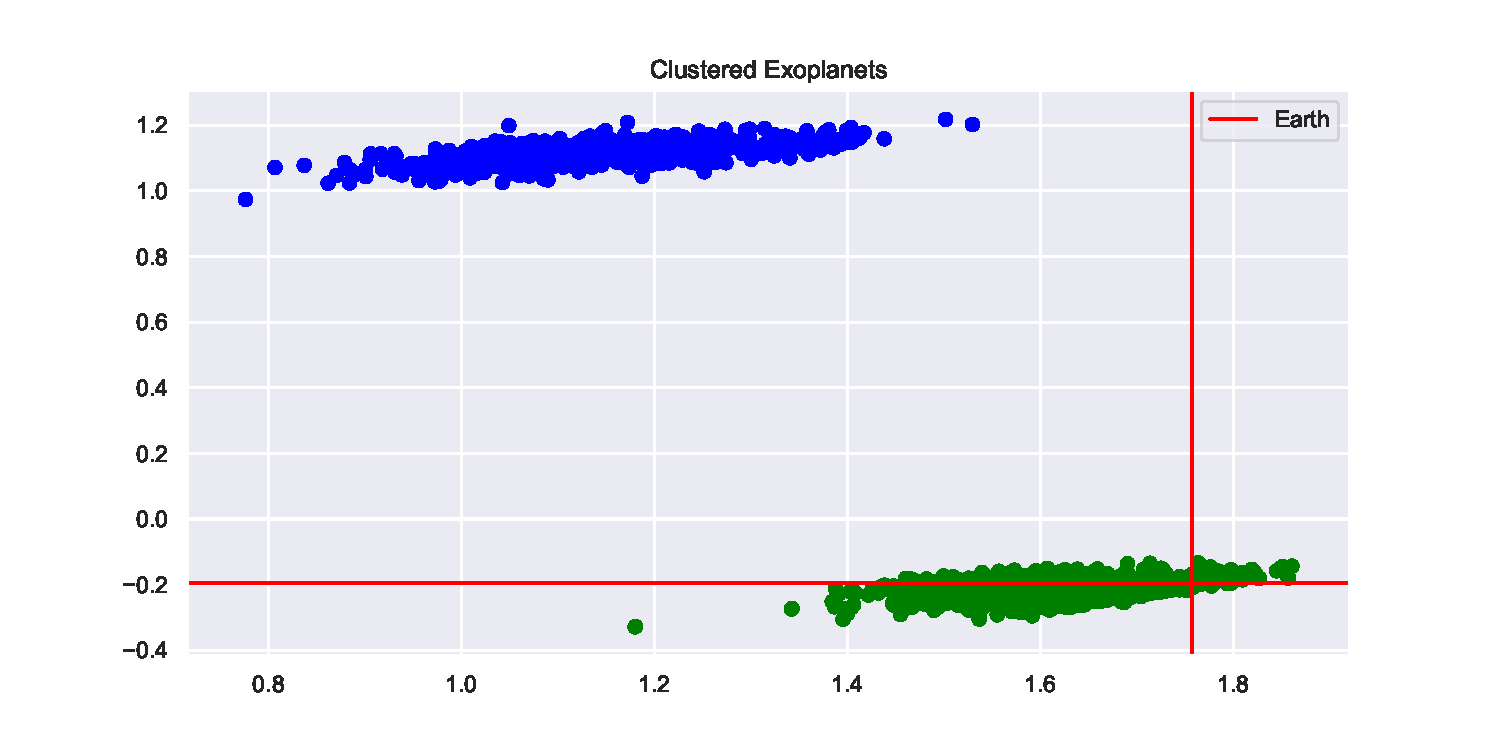
\includegraphics[width=0.9\textwidth]{graphics/cluster.pdf}
    \caption{K-Means Clustering the Exoplanets projected by SVD into 2 dimensions}
    \label{pic:cluster}
\end{figure}

%------------------------------------------------------------------

\section{Ranking}
The ranking is computed by evaluating the similarity of each exoplanet to the specs of planet Earth based on a the parameters we extracted beforehand such as the surface temperature of the planet, it’s gravity, it’s light exposition, etc. We believe that some parameters probably have a bigger impact than others on how ``livable`` an exoplanet is. For instance, the year of discovery of the planet is probably not as important as it's surface temperature or it's gravitational force. Therefore two rankings have been computed: There is one ranking that doesn't take into account the weight of the parameters, and one that does.

In the so-called weighted ranking, parameters will see themselves attributed a weight coefficient that goes from 0 to 10 , which influences the computed score and therefore results in a different rating. The importance factors that were associated with the attributes were introduced by our sense of understanding on what is important.

The Ranking is computed using the native python-embedded cosine similarity formula, where $u$ and $v$ are the vectors for on exoplanet data row, and $w$ the weight coefficient of a parameter.

\begin{align}
\text{cosine}(u,v) &= \frac{\sum_{i=0}^{n-1} u_iv_i  }{ \sqrt{\sum_{i=0}^{n-1} u_i^2  } \sqrt{\sum_{i=0}^{n-1} v_i^2  }} \label{eq:cosine}\\
\text{cosine}_{\text{weighted}}(u,v,w) &= \frac{\sum_{i=0}^{n-1} (u_i-\overline{u_w})(v_i-\overline{v_w})  }{ \sqrt{\sum_{i=0}^{n-1} (u_i-\overline{u_w})^2  } \sqrt{\sum_{i=0}^{n-1} (v_i-\overline{v_w})^2  }} \label{eq:cosine_weighted} \\
\overline{u_w} &= \frac{ \sum_{i=0}^{n-1} u_iw_i }{ \sum_{i=0}^{n-1} w_i } \label{eq:weighted_mean}
\end{align}

%------------------------------------------------------------------

\section{Webapp}
We then came up with a node.js web application to display the results of our ranking, This website uses native HTML/CSS/JS, a node.js templating engine to pass data to views as well as some data visualisation framework such as chart.js to make it easier to display our data.

The Webapp displays the ten first planets for both the weighted and unweighted ranking.

%------------------------------------------------------------------

\section{Results}
bla, bla,...

%------------------------------------------------------------------

\printbibliography

\appendix

\begin{landscape}
    \section{Dataset Attributes}
    \begin{table}[!h]\centering
        \caption{Attributes Description}
        \label{tab:att_desc}
        \begin{tabular}{|l l c|}\hline
            Attribute         & Description & Weight \\ \hline\hline
            fpl\_orbper      & orbital period (days) & 5 \\ \hline
            fpl\_smax        & the longest radius of an elliptic orbit & 3 \\ \hline
            fpl\_bmasse    & mass of the planet (earth unit) & 5 \\ \hline
            fpl\_rade         & radius (earth unit) & 5 \\ \hline
            fpl\_dens        & density of the planet (g/cm**3) & 7 \\ \hline
            fpl\_tranflag    & wether the lanet transits the star or not & 1 \\ \hline
            fpl\_cbflag      & does planet orbit a binary solar system & 5 \\ \hline
            fpl\_snum       & number of stars in the solar system & 8 \\ \hline
            dec                 & declination of the planetary system & 3 \\ \hline
            fst\_teff          & effective temperature in Kelvins & 10 \\ \hline
            fst\_logg        & gravity acceleration at the star surface log10(cm/s**2) & 4 \\ \hline
            fst\_lum         & star lumonisty log10(lumonisity) & 4 \\ \hline
            fst\_mass       & stellar mass (sun unit) & 6 \\ \hline
            fst\_rad         & stellar raidus (sun unit) & 6 \\ \hline
            fst\_met        & star metallicity & 3 \\ \hline
            fst\_metratio & metal abundance (in comparison to sun) & 1 \\ \hline
            fst\_age         & stellar age (in billions) & 8 \\ \hline
        \end{tabular}
    \end{table}
\end{landscape}

\section{Charts}

\begin{figure}[!ht]\centering
    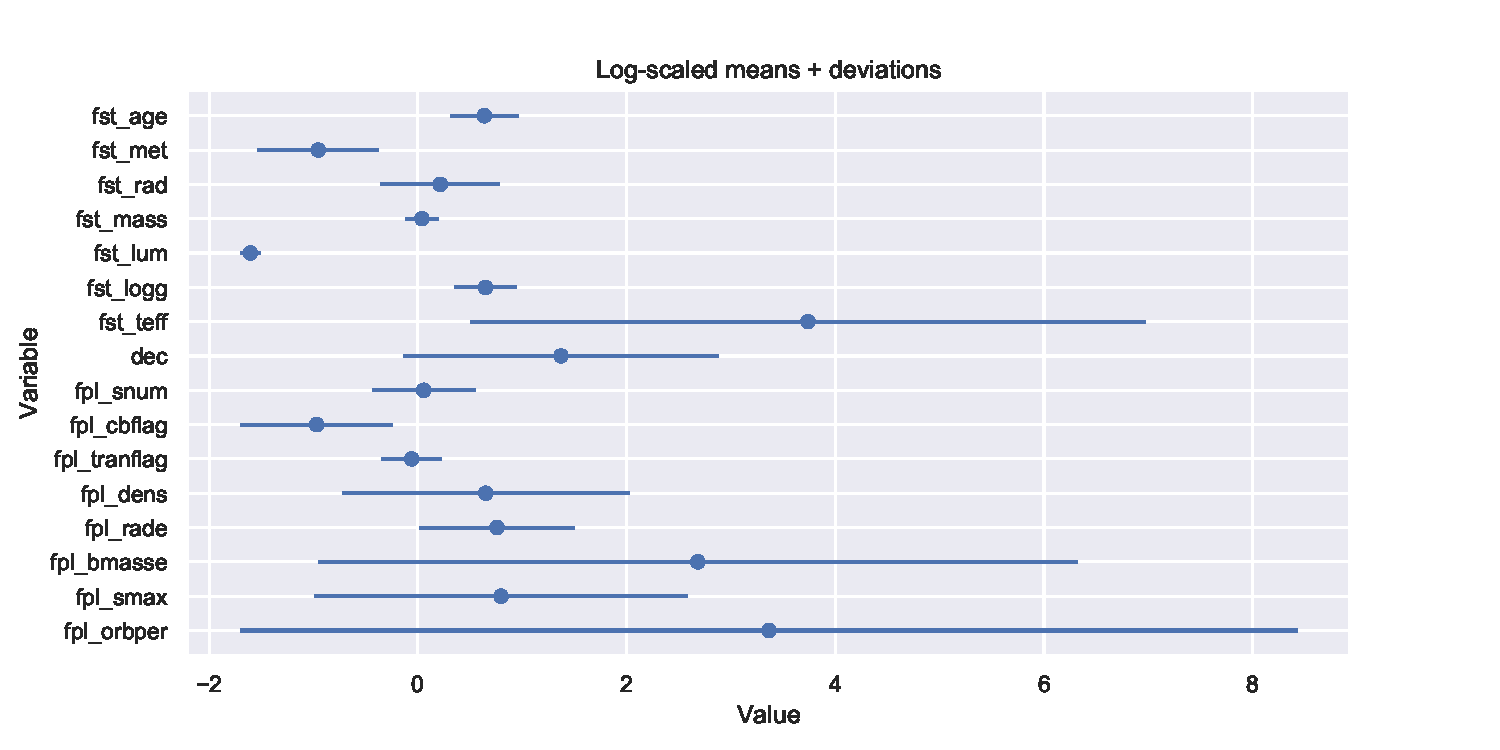
\includegraphics[angle=90, width=0.7\textwidth]{graphics/mean_deviation.pdf}
    \caption{log-scaled mean of each variable with its standard deviation}
    \label{pic:mean}
\end{figure}

\begin{figure}[!ht]\centering
    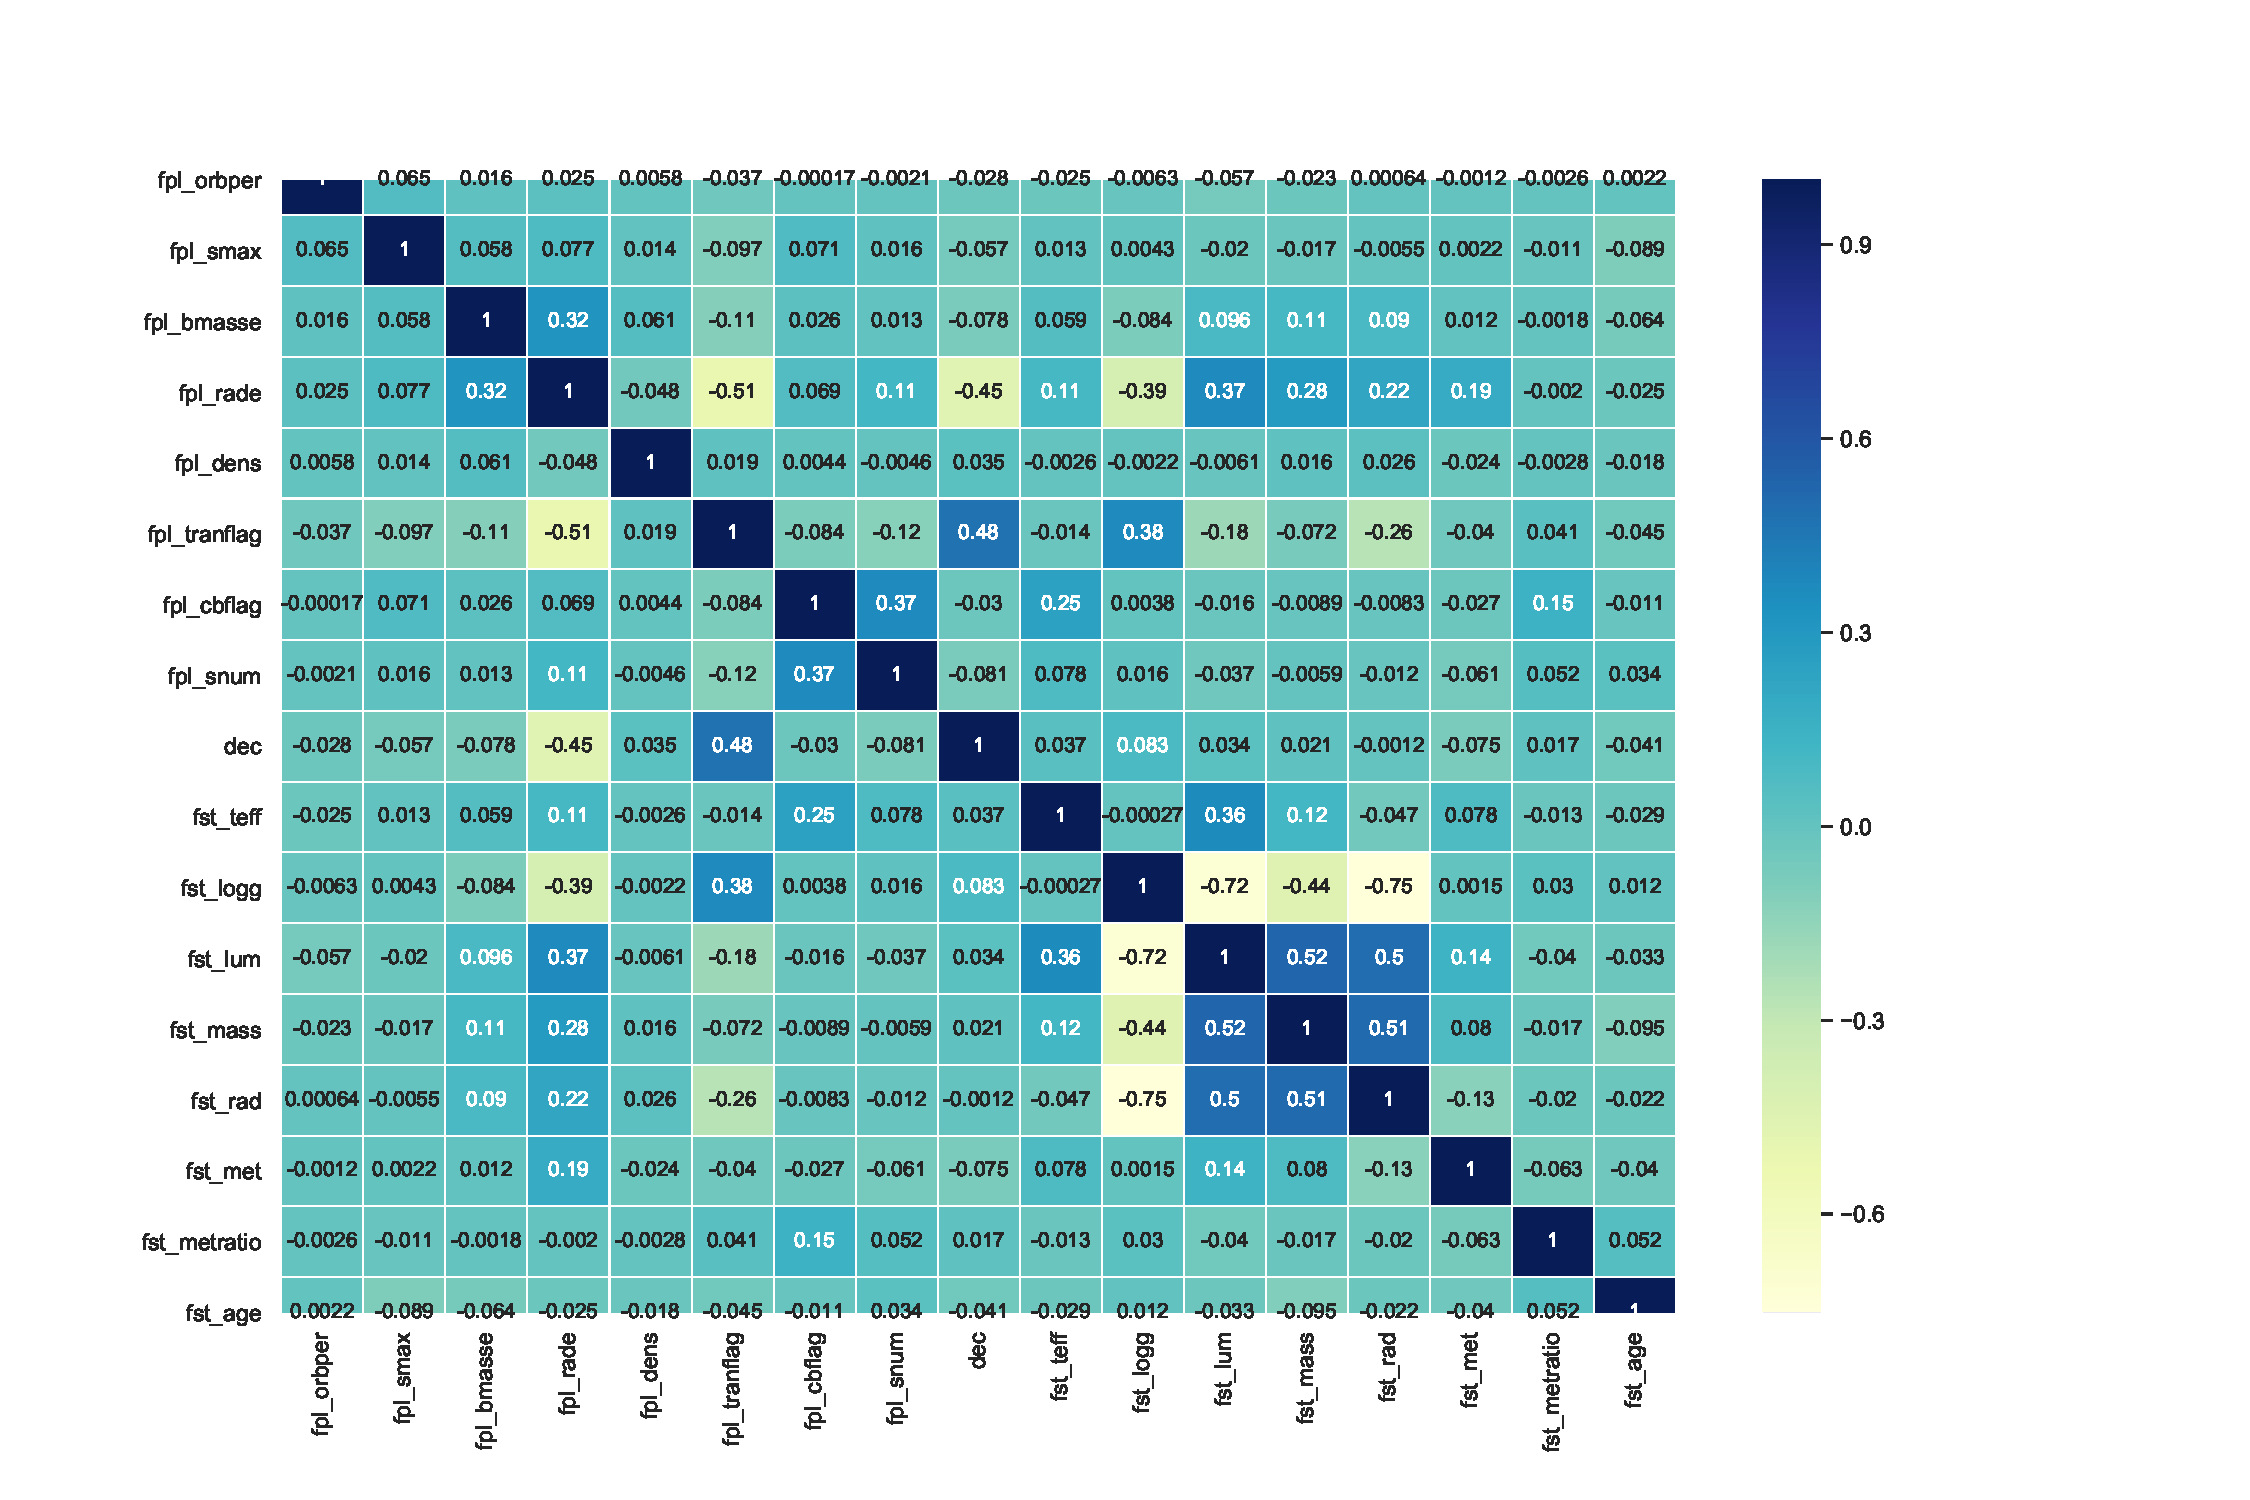
\includegraphics[angle=90, width=1\textwidth]{graphics/correlation_matrix.pdf}
    \caption{correlation matrix of variables}
    \label{pic:corr}
\end{figure}

\end{document}
